%!TEX root = ../../main.tex

\chapter{Silicon Vacancy Centers in Diamond}	\label{ch::sivs}
\chaptermark{SiV Centers}

  In the following we introduce \ccs, i.e.\ optically active point-defects present in a diamond lattice.
  We focus on \ccs combining silicon impurities and lattice vacancies forming the \sivc (\siv).
  We start by presenting the most important properties of diamond and emphasize its suitability as a host for optical applications with \ccs.
  A classification of diamond with respect to defects and impurities as well as crystallinities serves as a preparation for the introduction of methods to synthesize diamonds containing \sivs presented in \Fref{ch::fabrication_nanodiamonds}.
  Finally, we discuss \sivs in detail and focus on their most important optical properties which make them ideal candidates for realizing reliable \spss at room temperature.
  In particular, we zoom in on the key features of its luminescence spectrum, the \zpl and the \psb.
  Our discussion partially follows the presentation in \cite{Riedrich-moller2014, neu2012, BeckerMasterThesis, Steinmetz2011}.

\section{Diamond as a host lattice}

  Diamond is a metastable modification of carbon which is stable under normal pressure at room temperature \cite{Bundy1989}. Carbon atoms form strong sp$^3$-bonds with each other in a tetrahedral arrangement of neighboring atoms. For an extensive introduction of carbon bonds refer to \Fref{ch::crystal_quality}. The resulting sp$^3$-hybridized lattice is of exceptional mechanical stability, making diamond the hardest known material \cite{telling2000theoretical}.
  The crystal structure can also be interpreted as a face-centered cubic (fcc) lattice with two carbon atoms in the primitive Bravais cell, situated at $(0,0,0) \ a$ and $ (\frac{1}{4}, \frac{1}{4}, \frac{1}{4}) \ a$ with $a = \SI{3.567}{\angstrom}$ denoting the lattice constant \cite{Saotome1998}. \Fref{fig::diamond_lattice} illustrates the structure.

  \begin{figure}[htbp]
		\centering
		\testbox{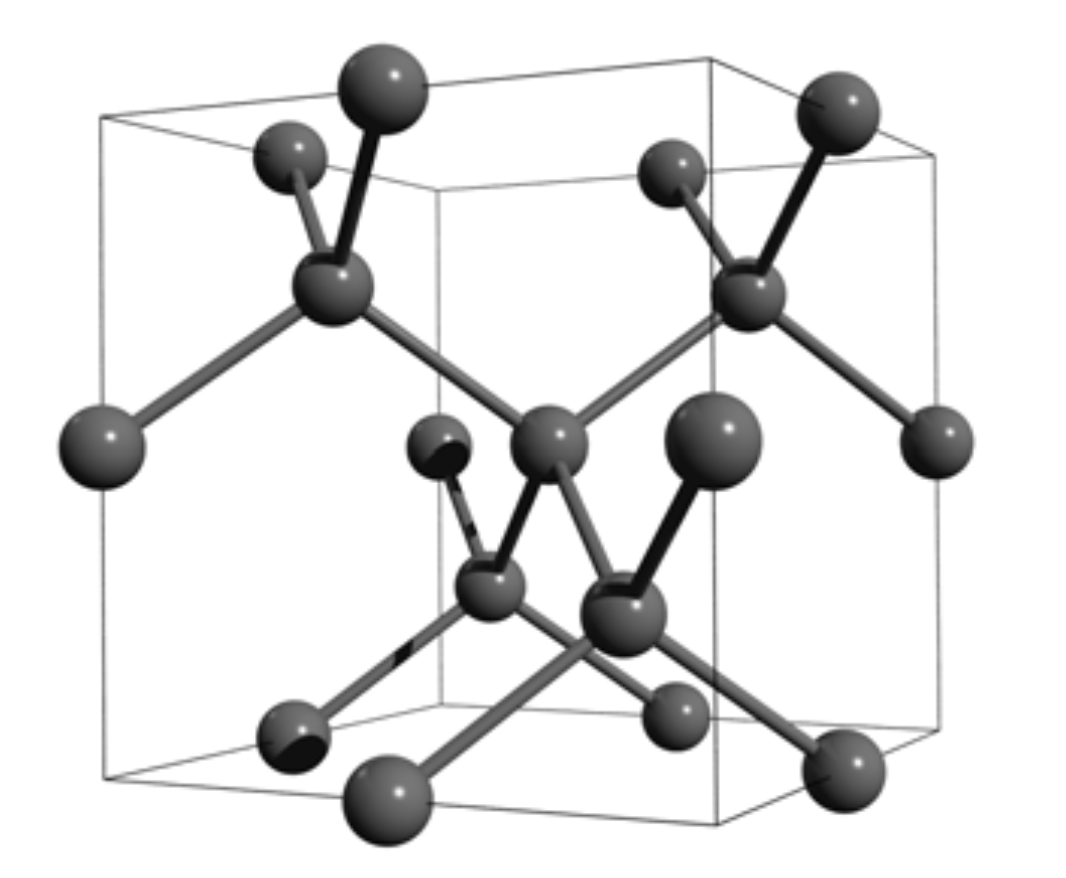
\includegraphics[trim = 0 0 0 0,  clip= true, width = 0.3\textwidth]{./pics/diamond_lattice.png}}
		\caption[Face-centered cubic diamond lattice]{Face-centered cubic diamond lattice. Note the tetrahedral arrangements of carbon atoms \cite{demtroder2000experimentalphysik}.}
		\label{fig::diamond_lattice}
	\end{figure}

  The valence and conduction bands of diamond are separated energetically by a large direct band gap of \SI{7.3}{\eV} while its indirect band gap amounts to \SI{5.5}{\eV} \cite{Clark1964, Saslow1966}. As a result diamonds are transparent for light of all wavelengths larger than \SI{230}{\nm} \cite{Mildren2008}. This transparent quality makes diamond an ideal host material for various optically active lattice defects or impurities. These induce a wide range of discrete energy levels situated in the sizable band gap. The absorption of optically active impurities or impurity complexes gives rise to the observed variety of colors in diamonds, thus these impurities are commonly termed color centers \cite{neu2012}. Due to the exceptional mechanical stability of diamond, color centers too are very stable mechanically, another important property favorable for optical applications.

  A property of diamond, detrimental to some optical applications, is its large refractive index with values of $2.49$ at \SI{360}{\nm} and $2.4$ at \SI{800}{\nm} respectively \cite{Zaitsev2001}. Thus, a portion of the light escaping from the diamond is reflected back into it, effectively reducing the efficiency of light extraction, see \Fref{subfig::diamond_refraction_bulk}. If \nds smaller than the \wl of the light to be collected are used, internal reflection is suppressed and the extraction efficiency can be increased \cite{Beveratos2001} as illustrated in \Fref{subfig::diamond_refraction_nd}. As a result, the quantum yield defined as the ratio between the number of photons emitted by the \siv to the number of photons absorbed by the diamond is enhanced.

  \begin{figure}[thbp]
    \begin{subfigure}[t]{ 0.49\linewidth}
      \centering
      \testbox{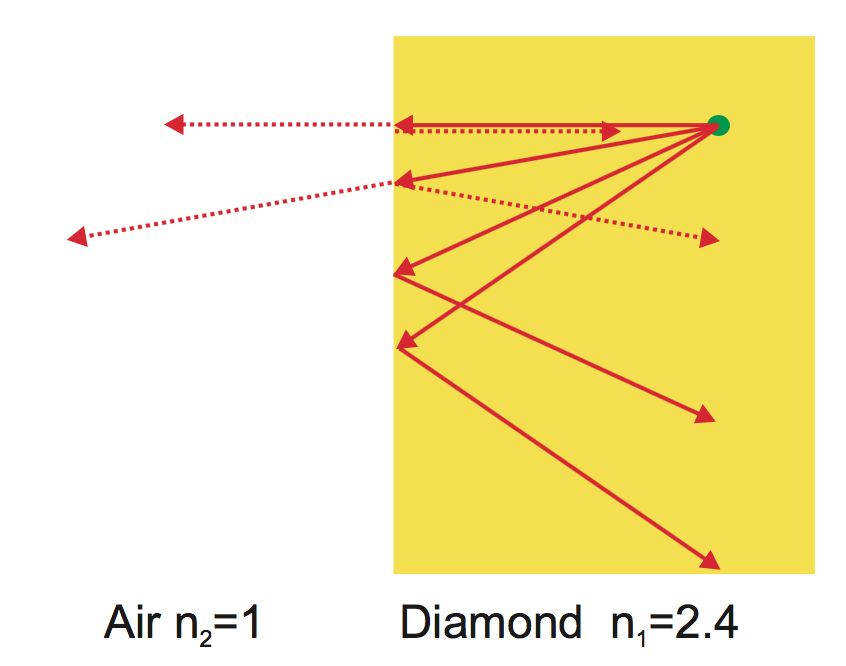
\includegraphics[trim = 0 0 0 0,  clip= true, width = 0.7\textwidth]{./pics/diamond_refraction.png}}
      \caption{}
      \label{subfig::diamond_refraction_bulk}
    \end{subfigure}
    \hfill
    \begin{subfigure}[t]{ 0.49\linewidth}
      \centering
      \testbox{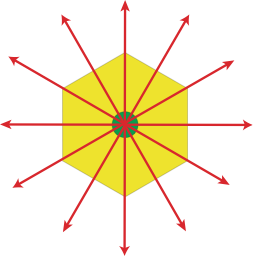
\includegraphics[trim = 0 0 0 0,  clip= true, width = 0.7\textwidth]{./pics/nanodiamond_-small-14626.png}}
      \caption{}
      \label{subfig::diamond_refraction_nd}
    \end{subfigure}
    \caption[Light extraction efficiency of diamond]{(a) Light from a fluorescent emitter inside the diamond (green dot) undergoes reflection at the diamond-air interface. Figure reproduced with permission from \cite{neu2012}. (b) Nanodiamond smaller than \fl \wl, reflection is suppressed.}
    \label{fig::extraction_efficiency}
  \end{figure}

\section{Classification of diamond}

  Two major approaches for classifying diamond are commonly encountered. First, classification according to the presence or absence of certain impurities or impurity complexes. Second, classification based on different diamond crystallinities observed in the diamond. In the following both classification systems are briefly introduced.

  \subsection{Classification by impurities}

    Impurities or complexes of impurities in the diamond lattice can be optically active and thus change the optical properties of diamond. Most strikingly perhaps is the appearance of color in otherwise colorless diamond due to a sufficient concentration of such defects. Using IR absorption spectroscopy the degree of nitrogen impurities can be determined. It is used to subdivide diamonds into distinct groups named Type I and Type II \cite{Kaiser1959, Breeding2009}. The groups are further subdivided as follows:

    \begin{itemize}
          \item Type Ia: With a nitrogen concentration of up to \SI{3000}{ppm}, most natural occurring diamonds belong to this group \cite{Zaitsev2001}. Nitrogen appears arranged predominantly in aggregate clusters forming complexes of impurities. These complexes are optically active, absorbing light in the blue range of the visible spectrum. Consequently Type Ia diamonds often exhibit a yellow to brownish coloration.

          \item Type Ib: With concentrations of up to \SI{500}{ppm}, nitrogen atoms appear predominantly in isolation, replacing individual carbon atoms in the diamond lattice. In addition to absorbing visible blue light, green is being absorbed as well. Type Ib diamond thus exhibits intensified yellow or brownish coloration. While only \SI{0.1}{\percent} of naturally occurring diamond fall into this class, almost all synthetic diamonds created using the \hpht (\HPHT) method are of Type Ib \cite{Zaitsev2001}.
    \end{itemize}

    While Type I diamond exhibits an appreciable concentration of nitrogen, Type II diamonds lack nitrogen entirely. Type II diamond is divided into two subgroups according to the presence or absence of boron as follows:

    \begin{itemize}
      \item Type IIa: Can be considered pure as they lack boron impurities and other optically active defects \cite{Walker1979}. They thus are colorless. Up to \SI{2}{\percent} of naturally occurring diamond and most diamonds synthetically created using the \cvd (\CVD) method are of Type IIa \cite{Zaitsev2001}.
      \item Type IIb: Contains appreciable concentrations of boron atoms replacing individual carbon atoms in the diamond lattice. Boron defects are optically active absorbing visible light ranging from red to yellow. Depending on the Boron concentration blue to gray colorations are observed. Furthermore, diamond changes from an insulator to an efficient $p$-type semiconductor in the presence of boron impurities \cite{Massarani1978}.
    \end{itemize}

    We remark that for many modern applications of diamonds the presented ``classic" categorization of diamond is insufficient. In these cases a precise quantification of the concentration and nature of various relevant impurities is called for \cite{Markham2011, Balasubramanian2009}.

    In this section we also briefly touched upon the \CVD and \HPHT methods, two approaches to synthetically produce diamonds. Both are relevant for this thesis and are explained in detail in \Fref{ch::fabrication_nanodiamonds}.

  \subsection{Classification by crystallinity}

    Up until now, the discussion assumed that diamond forms a lattice consisting of one giant single crystal. However, other crystallinities are possible and can be used to classify diamond.
    They range from mono or single crystals to polycrystalline, nanocrystalline or even ultra-nanocrystalline diamond films \cite{May2000}. This classification is particularly useful for synthesized diamond as will be discussed in \Fref{ch::fabrication_nanodiamonds}. \Fref{tab::diamond_grain_sizes} summarizes the different sizes of diamonds or diamond films which can be achieved using variations of the \CVD method. In the context of this thesis it is not necessary to distinguish \nds based on the size of their crystallinities, it suffices to distinguish between mono- and polycrystalline \nds. 

    Diamond films consist of isolated diamond grains of random orientation with sp$^2$ hybridized grain boundaries and graphite-like inclusions \cite{Riedrich-moller2014}. Carbon present in non-diamond phases, e.g.\ graphite or amorphous carbon gives rise to detrimental light absorption while crystal boundaries lead to increased scattering losses. As the size of diamond crystallites get smaller, the ratio of non-diamond carbon to diamond carbon increases. Thus losses are most pronounced for the smallest grain diamond films. 

    \begin{table}[htbp]
  		\centering
  		\caption[Classification of diamond synthesized by \cvd]{Classification of diamonds synthesized using \CVD \cite{Steinmetz2011}.} \label{tab::diamond_grain_sizes}
  			\begin{tabular}{lc}
  			\toprule
  			Crystallinity & Grain size  \\
  			\midrule
  			monocrystalline & arbitrary \\
  			polycrystalline & \SI{50}{\nm} to \SI{10}{\micro\meter} \\
  			nanocrystalline & \SI{10}{\nm} to \SI{50}{\nm} \\
  			ultra-nanocrystalline & $<$ \SI{10}{\nm} \\
  			\bottomrule
  			\end{tabular}
  	\end{table}

\section{The \Sivc} \label{sec::siv}

  A \cc is an optically active point-defect in a crystal lattice, capable of absorbing and emitting light. Defects can consist of one or several vacant lattice sites, foreign atoms replacing lattice atoms or a combination thereof. If the presence of a defect induces discrete energy levels located in the band gap of the host material, the \cc can be interpreted as its own quantum system. In other words, the \cc can be viewed as a single isolated and localized artificial atom embedded in a host matrix. As such it is able to absorb light and emit single photons by means of fluorescence.

  Compared to alternative single photon sources like single atoms \cite{Kuhn2002}, ions \cite{Keller2004} or individual quantum dots \cite{Michler2000, Yuan2002}, \ccs offer a couple of advantages due to their solid state environment. As a result of the high mechanical stability of the host lattice \ccs exhibit increased photo-stability, in particular compared to organic molecules as light sources. Furthermore the host lattice offers protection of \ccs from detrimental interactions with aggressive free molecules \cite{Lounis2005}. Lastly, \ccs can be handled and investigated at room temperature and ambient pressure, thus significantly reducing the experimental sophistication necessary to study them.

  Of particular interest are \ccs as single photon sources when hosted in diamond. With its transparency, exceptional stability and minimal phononic interactions at room temperature the diamond lattice is an ideal host matrix for \ccs \cite{Kennedy2003,Greentree2008}. While more than $500$ different \ccs in diamond are documented, only a small fraction has been investigated with respect to their properties as \spss \cite{Zaitsev2001}. For an in-depth review of \ccs and their versatile applications see \cite{Aharonovich2014, Prawer2014}. The two arguably most prominent examples of well-studied \ccs are vacancy centers featuring nitrogen and silicon \cite{Manson2006, Jelezko2002, Santori2006}.

  The \sivc (\siv) in diamond and its properties is at the center of this thesis. The \siv has been established as a reliable single photon source at room temperature. It shows very narrow emission lines with record count rates on the order of mega-counts-per-second \cite{Neu2012a}. The emission of indistinguishable photons and the optical access of electronic spin states have been demonstrated \cite{Sipahigil2014, Mueller2014, Pingault2014, Rogers2014a}, hinting at the possibility of deploying \sivs as spin-qubits.

  A \sivc is formed in a diamond lattice by substituting two carbon atoms by a silicon atom and a nearby empty lattice site respectively. The silicon atom occupies its energetically optimal position by sitting in-between two lattice sites. This is called ``split-vacancy'' configuration and induces a $D_{3d}$ symmetry with the two vacancies and the impurity aligned along the $\langle 111 \rangle$ diamond axis \cite{goss2007density}, see \Fref{fig::siv_lattice}.

  \begin{figure}[htbp]
		\centering
		\testbox{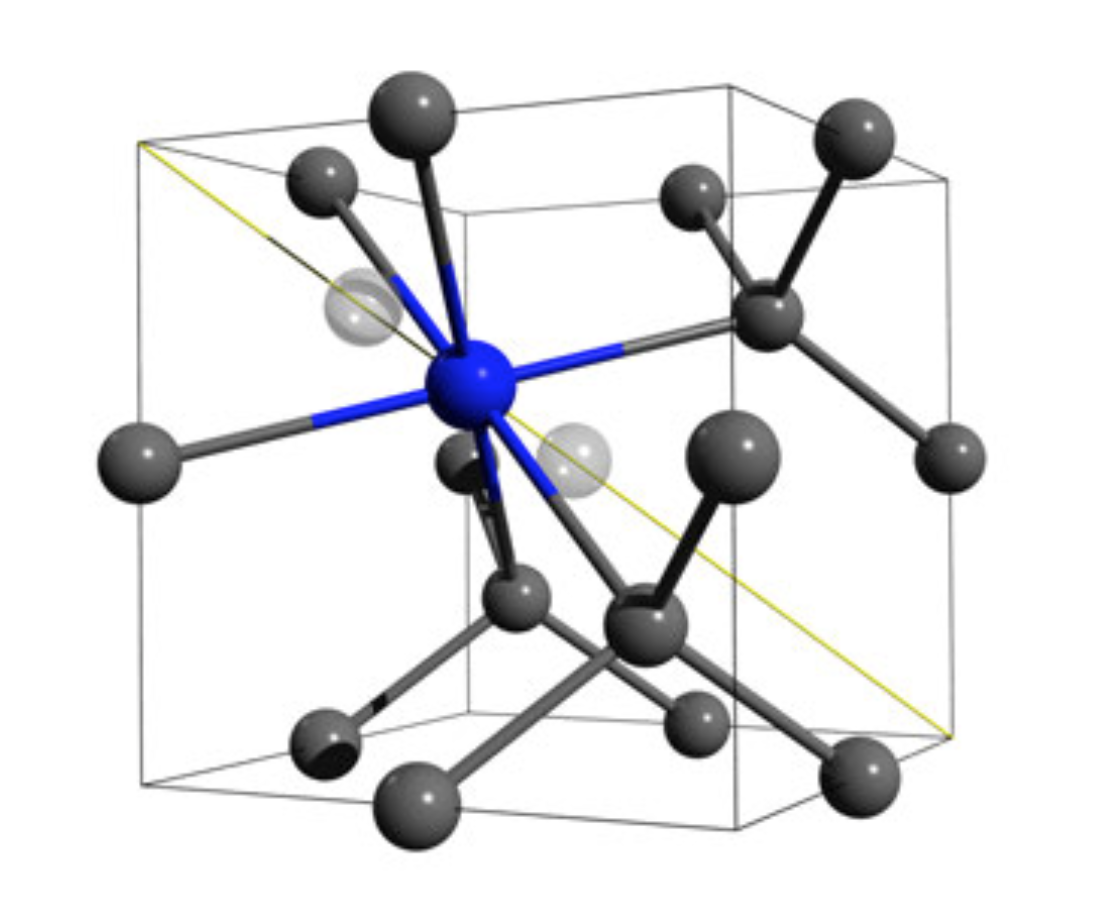
\includegraphics[trim = 0 0 0 0,  clip= true, width = 0.3\textwidth]{./pics/siv_lattice.png}}
		\caption[Split-vacancy configuration for \sivs in diamond]{Crystal structure of the \siv embedded into the diamond lattice: The silicon atom (blue sphere) sits in between two vacant lattice sites (white spheres) forming a ``split-vacancy'' configuration aligned along the $\langle 111 \rangle$ crystallographic axis (yellow line). Figure reproduced with permission from \cite{Riedrich-moller2014}.}
		\label{fig::siv_lattice}
	\end{figure}


  The \siv is known to occur in two different charge states. The first is the neutral state or SiV$^0$ with a zero-phonon transition at \SI{1.31}{\eV} (\SI{946}{\nm}). It is associated with a $S = 1$ ground state \cite{DHaenens-Johansson2011}. The second state is the negatively charged state SiV$^{-}$ where the \sivc recruited an additional free electron. It exhibits a zero-phonon transition at \SI{1.68}{\eV} (\SI{738}{\nm}). Its ground state has been determined as a $S = \frac{1}{2}$ state \cite{Goss2007, Hepp2014}. Due to its outstanding brightness and the location of the \zpl in the visible range of the spectrum, this thesis focuses on the negatively charged \siv. For convenience we drop the charge distinction from now on and refer to SiV$^{-}$ centers simply as \sivs.

  \sivs are synthesized using \CVD in \nds and single-crystal diamond films \cite{Neu2011b}, see \Fref{ch::fabrication_nanodiamonds} for details. It is also possible to directly implant silicon atoms into diamond. After the implantation, high temperature annealing must be used to animate present lattice vacancies to recombine with silicon impurities in order to form split-vacancy \sivs \cite{Collins1983,Hepp2014}.

  In the following sections we detail the most important luminescence properties of \sivs in diamond. For a comprehensive review we refer to \cite{Riedrich-moller2014, neu2012} and references therein.


  \subsection{Luminescence properties}

    The \sivc as a quasi-atomic system is capable of absorbing and emitting light. When a ground state electron absorbs a photon of appropriate energy, it is promoted to a discrete higher-energy excited state located within the band gap of the diamond host matrix. Reversing this excitation relaxes the electron back down to the ground state while emitting a so-called fluorescent photon, accounting for the energy difference between excited and ground state. This transition is ``spin-allowed", limiting the life-times of excited states to nanoseconds and thus promoting rapid relaxation and associated fluorescence \cite{Gali2013b}.

    Fluorescence is directly linked to the electronic structure of the \siv, see \Fref{fig::above_resonant_excitation}. It follows that photoluminescence spectroscopy can be used to study it using a laser to optically excite the \siv. In the context of this thesis, optical above-resonant excitation is the method of choice, in particular, when used in conjunction with a confocal photoluminescence setup which will be discussed in \Fref{ch::pl_setup}.
    If the excitation energy exceeds the energy of the lowest excited state, electrons are promoted to higher electronic and vibrational states. Conveniently, these states relax rapidly towards the lowest exited state in non-radiative processes \cite{Gali2013b}. Once the lowest excited state is reached, a florescent transition to one of the ground state levels can follow \todo{Insert explanation of saturation and decay rate}. It has been shown that above-resonant excitation is feasible for excitation energies ranging from \SIrange{1.75}{2.55}{\eV} \todo{Insert wavelengths in addition to energies} \cite{iakoubovskii2001optical, Iakoubovskii2000, Rossi1997}. If the excitation energy is chosen too high, however, the \siv is ionized. This is unfavorable, since electrons escaping to the diamond conduction band do no longer induce fluorescence. Ionization may be reversed if an \siv manages to capture a free electron from the conduction band. This charge state conversion is believed to be linked to fluorescence intermittence, describing ``blinking'' \sivs \cite{Muller2011, Siyushev2009}.

    \begin{figure}[htbp]
      \centering
      \testbox{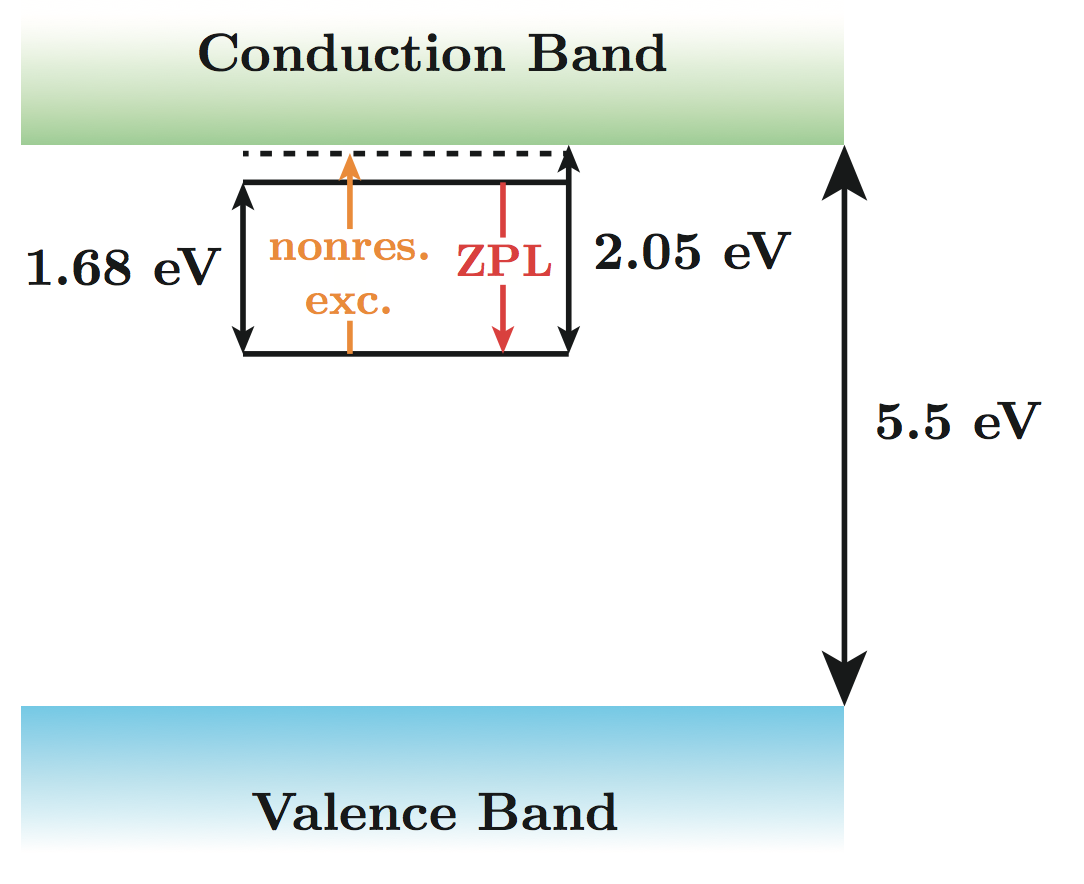
\includegraphics[trim = 0 0 0 0,  clip= true, width = 0.3\textwidth]{./pics/above_resonant_excitation.png}}
      \caption[Band gap of \sivs hosted in diamond]{Simplified picture of the generous \SI{5.5}{\eV} band gap of diamond with discrete states induced by the presence of \sivs. The \siv ground state is situated \SI{2.05}{\eV} below the diamond conduction band. The lowest excited state sits \SI{1.68}{\eV} above the ground state with the \zpl transition in red connecting the two. Above-resonant optical excitation is indicated in orange. Figure courtesy of \cite{BeckerMasterThesis}.}
      \label{fig::above_resonant_excitation}
    \end{figure}

    The fluorescence spectrum of \sivs typically show two prominent features: A narrow \zpl a weak \psb. The former is connected to fluorescent photons associated with a purely electronic transition while the latter involves vibrational transitions involving electron-phonon interactions. The \psb is typically shifted to higher \wl, i.e.\ lower energies, with respect to the \zpl. The resulting energy deficit can be explained by phonons being created during the relaxation of higher vibrational states. A shift in the opposite direction can also be observed in rare cases if preexisting phonons are absorbed during the relaxation process \cite{Iakoubovskii2000thesis}.

    The relative strength of the \zpl and the \psb is influenced by electron-phonon coupling. Phonons can either originate locally, i.e.\ directly connected to the \siv, or delocalized connected to lattice vibrations. In the following we discuss localized phonon modes. For a discussion of delocalized modes we refer the reader to \cite{Feng1993b}. 

    When a \cc is excited, its charge distribution changes. As a result, the equilibrium positions of all particles involved in the \cc shift leading to slight changes in \cc geometry. Naturally, the combined changes of charge distribution and geometry of the \cc also affect the positions of surrounding atoms of the host lattice. Similarly, if the exited state relaxes back to the ground state, the process occurs in reverse. Thus, due to differing atomic arrangements for ground and exited states, the periodic emission and absorption of photons is accompanied by lattice vibrations, i.e.\ phonons. In other words, the electron-phonon interaction couples the motion of the lattice and electronic transitions of a color center \cite{Davies1981, Zaitsev2000}.

    The Huang-Rhys model allows us to discuss the electron-phonon interaction in \sivs in more detail.
    We remark at this point, that our discussion based on the Huang-Rhys model assumes that only one vibrational mode couples to the \cc which is a strong assumption. In general it is believed that in a solid state host matrix a discrimination between the modes of the undisturbed lattice and quasi-local impurity-induced modes is appropriate \cite{Zaitsev2000, Feng1993b, Solin1970}. Furthermore, various mechanical properties such as stress in the lattice are reported to affect phonon energies \cite{Grimsditch1978}. In addition, electron-phonon interactions and thus \psb features are believed to depend strongly on various local properties of \ccs \cite{Sternschulte1994, Huttner1995}. Thus it is possible to encounter complex varying \psb features from one \siv to the next. For a more detailed discussion of these effects we refer the reader to \cite{neu2012, Riedrich-moller2014} and references therein.

    Our discussion of the Huang-Rhys model follows the presentation in \cite{Doherty2013}. The model assumes in its simplest form that vibrational modes can be viewed as oscillations of nuclei between their equilibrium coordinates $q$ associated with the electronic states \cite{Riedrich-moller2014}. Let $\mathcal{K}_{{}^{3}A_{2}}(q)$ and $\mathcal{K}_{{}^{3}E}(q)$ denote the harmonic potentials of the ground and excited states respectively:

    \begin{align}
      \mathcal{K}_{{}^{3}A_{2}}(q) & = \frac{1}{2} \Omega^2 q^2 \\
      \mathcal{K}_{{}^{3}E}(q) & = C_{{}^{3}E} + aq + \frac{1}{2} (\Omega^2 + b)q^2 \\
       & = C_{{}^{3}E} - C_R + \frac{1}{2} (\Omega^2 + b)(q - \delta q)^2.
    \end{align}

    It follows that the vibrational modes of ground and exited states are given as harmonic states with discrete energies $\hbar \Omega (\nu + 2)$ as well as $\hbar \sqrt{\Omega + b} (\nu + 2)$ respectively, where $\nu$ denotes the occupation number and $\Omega$ the frequency.
    Further, let $aq$ denote the linear nuclear displacement of the excited state configuration with respect to the ground state equilibrium where $q = 0$ holds.
    The quadratic term $bq^2$ refers to the vibrational frequency shift due to a redistribution of charge between the electronic states.
    Given the linear and quadratic electron-phonon coupling strengths $a$ and $b$, the equilibrium displacement of the ${}^{3}E$ state can be obtained as:

    \begin{equation}
      \delta q = \frac{-a}{\Omega^2 + b },
    \end{equation}

    while the relaxation energy reads \cite{Doherty2013}:

    \begin{equation}
      C_R = \frac{a^2}{2 (\Omega^2 + b)} = \hbar S \sqrt{\Omega + b},
    \end{equation}


   where $S$ is referred to as Huang-Rhys factor.

   \begin{figure}[htbp]
     \centering
     \testbox{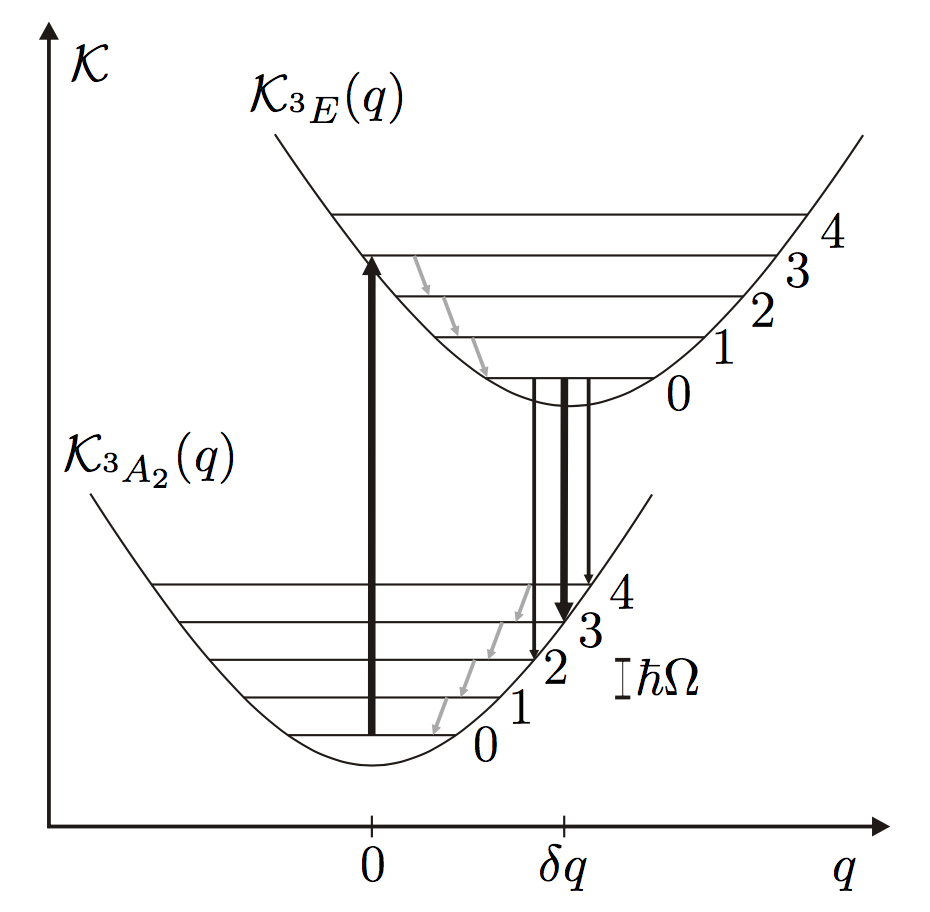
\includegraphics[trim = 0 0 0 0,  clip= true, width = 0.3\textwidth]{./pics/huang_rhys_model.png}}
     \caption[Huang-Rhys model of vibrational transitions]{Huang-Rhys model of the vibrational transitions in the Frank-Condon picture: The excited state $\mathcal{K}_{{}^{3}E}(q)$ is shifted by $\delta q$ with respect to the ground state potential $\mathcal{K}_{{}^{3}A_{2}}(q)$. The recombination originating at $\delta q$ marks the most probable transition (thick black arrow) from the fundamental ${}^{3}E$ vibrational level to one of the vibrational levels of the ${}^{3}A_{2}$ ground state followed by non-radiative transitions to the equilibrium position $q = 0$. The number of vibrational quanta involved in an optical transition are determined by the Huang-Rhys factor $S$. The excitation reverses the process. Optical transitions occur between states with identical values of $q$ and are shown as vertical black arrows. Non-radiative transitions change the value of $q$ and are shown as angled gray arrows. Figure and caption reproduced with permission \cite{Riedrich-moller2014}.}
     \label{fig::huang_rhys_model}
   \end{figure}

   To reason about the probabilities of various transitions between different vibrational levels associated with ground and excited states, the Franck-Condon principle can be applied \cite{condon1947franck}. It states that transitions between electronic states become more probable if origin and destination states have vibrational levels with similar energy. This implies that the most probable transitions occur between states requiring no change of nuclei positions. \Fref{fig::huang_rhys_model} illustrates the application of the principle for the Huang-Rhys model.

   We find that the most probable optical relaxation from an ${}^{3}E$ excited state back to an ${}^{3}A_{2}$ ground state originates from the fundamental vibrational ${}^{3}E$ state, \i.e.\ the lowest-energy excited state. This state is shifted by $\delta q$ with respect to the ground state, indicating that the energetically optimal nuclei positions differ from their ground state equilibrium positions. The most probable destination for the electronic relaxation process is a higher vibrational level of the ${}^{3}A_{2}$ ground state with similar nuclei positions. From there, electron-phonon interactions continue the relaxation process down to the fundamental vibrational level of the ground state. This non-radiative process allows nuclei to return to their original ground state equilibrium positions.
   The process of exciting the system from the ground state, proceeds in reverse. The most probable optical excitation promotes an electron from the fundamental ${}^{3}A_{2}$ ground state to a higher vibrational level of the ${}^{3}E$ excited state. The optical transition is such that nuclei positions do not change. Note that optical transitions are faster than vibrational transitions since they do not require a change in positions of massive nuclei. Once in the higher vibrational excited state, electron-phonon interactions mediate a transition down to the fundamental ${}^{3}E$ excited state with an associated change in nuclei positions. From there the relaxation-excitation cycle and its induced periodic changes in nuclei positions repeats.

   As discussed, transitions involving phonons mostly originate from the fundamental vibrational level of excited electronic states and end in higher vibrational states of the electronic ground state. Photons emitted during the relaxation process are associated with the \psb of the \siv.
   The observed red-shift of the \psb is directly tied to the phonon energy with higher order sidebands showing multiples of this energy. Note that the Huang-Rhys factor $S$ can be interpreted as an indicator of the most probable optical transition involving photons. Thus, it can be used to quantify the strength of the electron-phonon interactions in \sivs. A small value of $S$ indicates a weak electron-phonon coupling resulting in negligible \psb emissions. If no phonons are involved, the entire emission is concentrated in the \zpl. Conversely, a large value of $S$ indicates extensive electron-phonon interactions, leading to a pronounced \psb and a weaker \zpl. This dependence is naturally described by

   \begin{equation}
     S = -\ln{\frac{I_{ZPL}}{I_{ZPL} + I_{PSB}}}.
   \end{equation}

   For \sivs hosted in polycrystalline diamonds the Huang-Rhys factors have been determined to be very small ranging from \SIrange{0.08}{0.24}{} \cite{Duligall2006,Yuan2002,Nothaft2012}. As a result the \zpl as the most probable transition dominates the luminescence spectrum making \sivs excellent narrow-band emitters. \Fref{fig::spectral_features} illustrates the stark difference between the \zpl and the \psb. In contrast, $S=3.74$ has been established for nitrogen vacancy centers \cite{Davies1981}. A electron-phonon coupling of this magnitude concentrates almost all emission into the \psb and leaves the \zpl strongly suppressed.

   \begin{figure}[thbp]
 		\begin{subfigure}[t]{ 0.49\linewidth}
 			\centering
 			\testbox{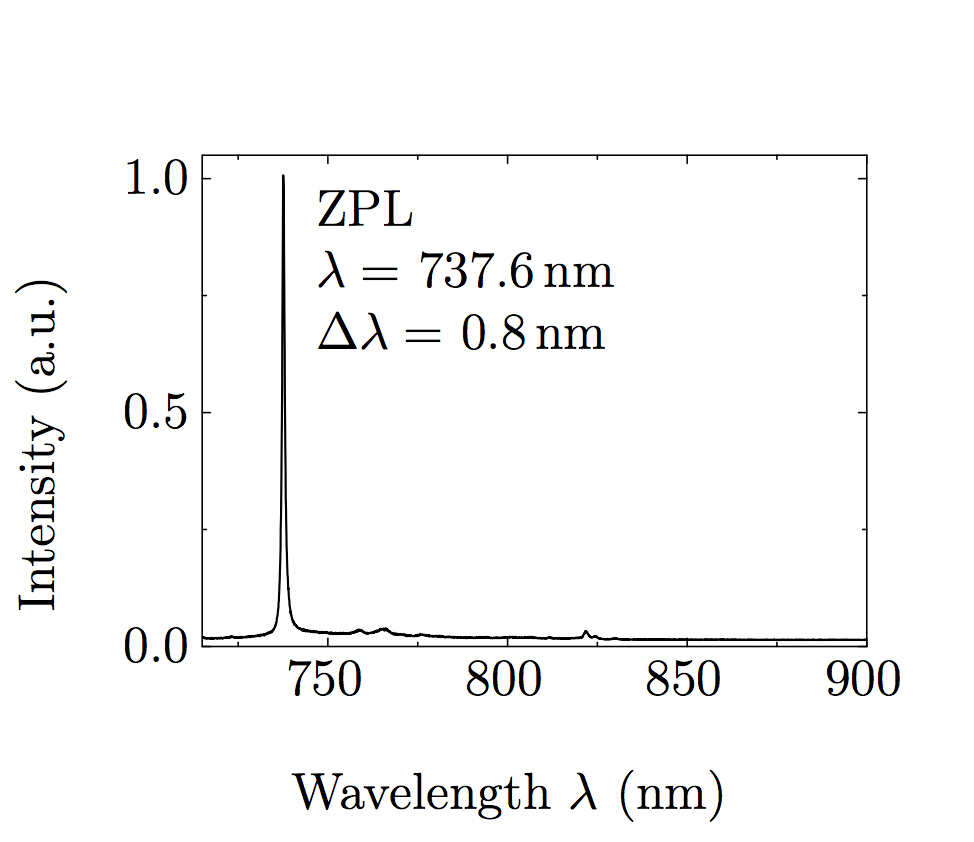
\includegraphics[trim = 0 0 0 0,  clip= true, width = 0.7\textwidth]{./pics/siv_zpl.png}}
 			\caption{}
 		\end{subfigure}
 		\hfill
 		\begin{subfigure}[t]{ 0.49\linewidth}
 			\centering
 			\testbox{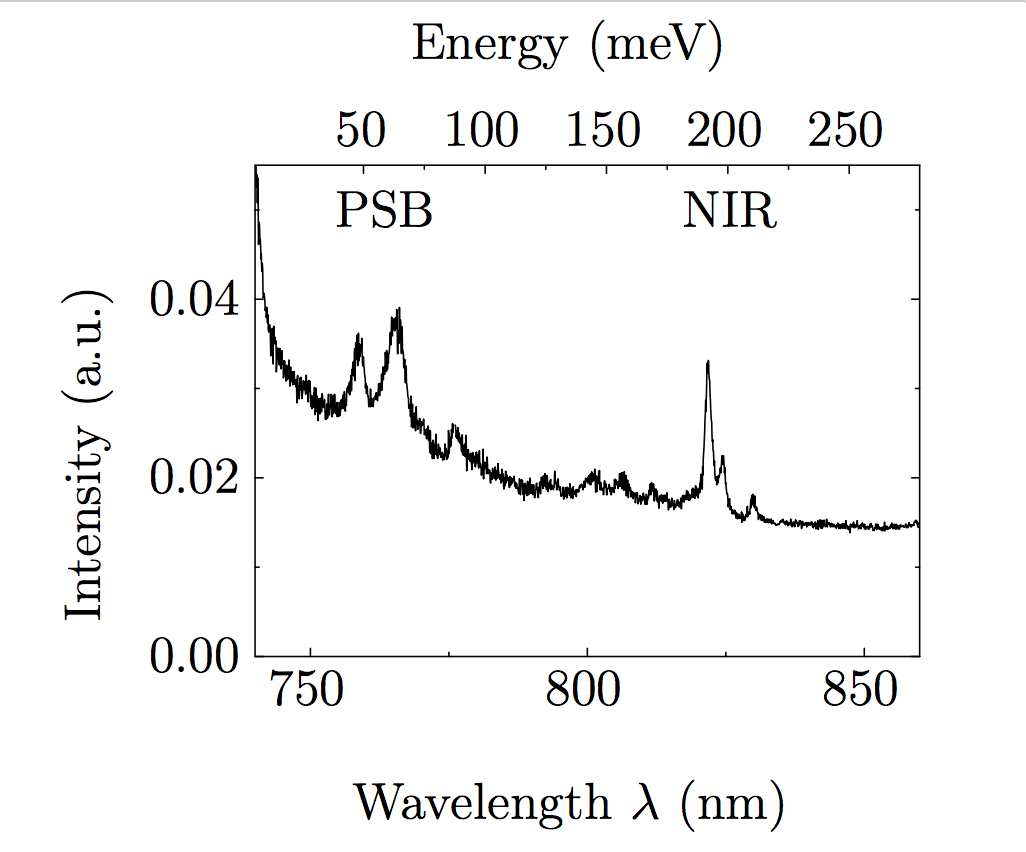
\includegraphics[trim = 0 0 0 0,  clip= true, width = 0.7\textwidth]{./pics/siv_sideband.png}}
 			\caption{}
 		\end{subfigure}
 		\caption[Fluorescence spectra of \sivs at room temperature]{(a) The narrow \zpl dominates the luminescence spectrum. (b) Low intensity \psb shows distinct vibrational transitions. Figure reproduced with permission \cite{Riedrich-moller2014}.}
 		\label{fig::spectral_features}
 	\end{figure}


   As an alternative measure for the electron-phonon coupling the Debeye-Waller factor can be used. It is closely related to the Huang-Rhys factor $S$ and defined as

   \begin{equation}
     D_w = e^{-S} = \frac{I_{ZPL}}{I_{ZPL} + I_{PSB}},
   \end{equation}

    which can be interpreted as the fraction of total photons that are emitted into the \zpl.

    We close this chapter with a short discussion of the luminescence spectra of \sivs at cryogenic temperatures. Naturally as temperatures approach absolute-zero the \psb must disappear since phonon creation ceases. If ensembles of \sivs are cooled below $\approx$ \SI{110}{\kelvin} a fine structure is revealed \cite{neu2013low}. It includes up to $12$ different lines with intensities proportional to the natural abundance of the three stable isotopes of silicon ${}^{28}Si, {}^{29}Si, {}^{30}Si$ \cite{Clark1995}. Each isotope is associated with $4$ lines attributed to doublet levels of ground and excited states which are split by \SI{0.2}{\milli\eV} and \SI{1.07}{\milli\eV} respectively \cite{Rogers2014, Hepp2014, Clark1995}. The splitting itself is believed to be a result of spin-orbit coupling with a weak contribution of the dynamic Jahn-Teller effect \cite{Hepp2014}. Initial results were based on ensembles of \sivs, however, recently the splitting was detected for isolated \sivs as well \cite{Dietrich2014a}. \Fref{fig::cryogenic_spectra} shows exemplary spectra representative for ensembles and single \siv at cryogenic temperatures.

    \begin{figure}[thbp]
  		\begin{subfigure}[t]{ 0.49\linewidth}
  			\centering
  			\testbox{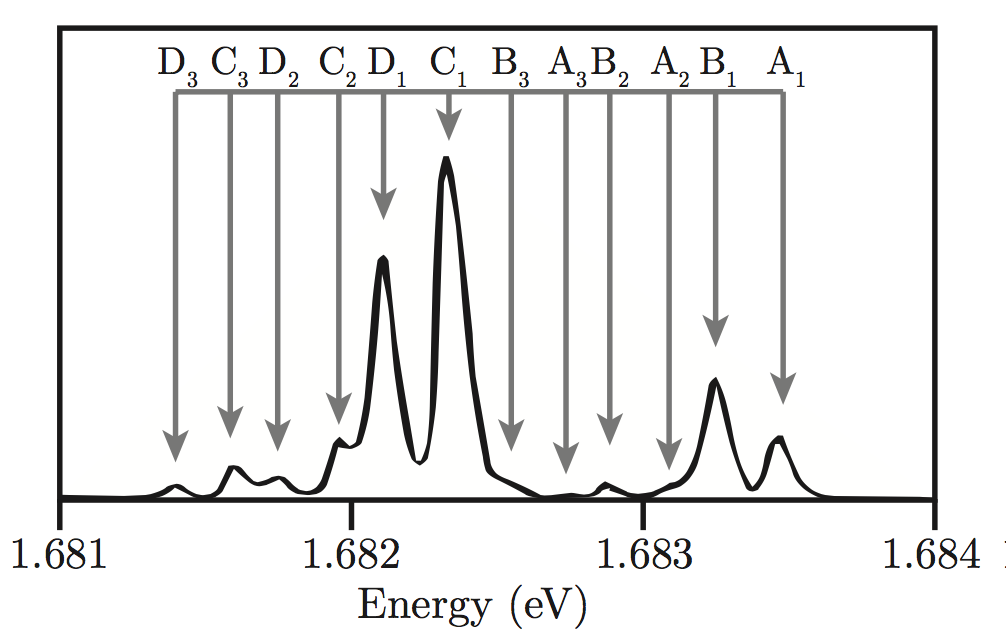
\includegraphics[trim = 0 0 0 0,  clip= true, height = 0.6\textwidth]{./pics/cryogenic_ensemble.png}}
  			\caption{}
  		\end{subfigure}
  		\hfill
  		\begin{subfigure}[t]{ 0.49\linewidth}
  			\centering
  			\testbox{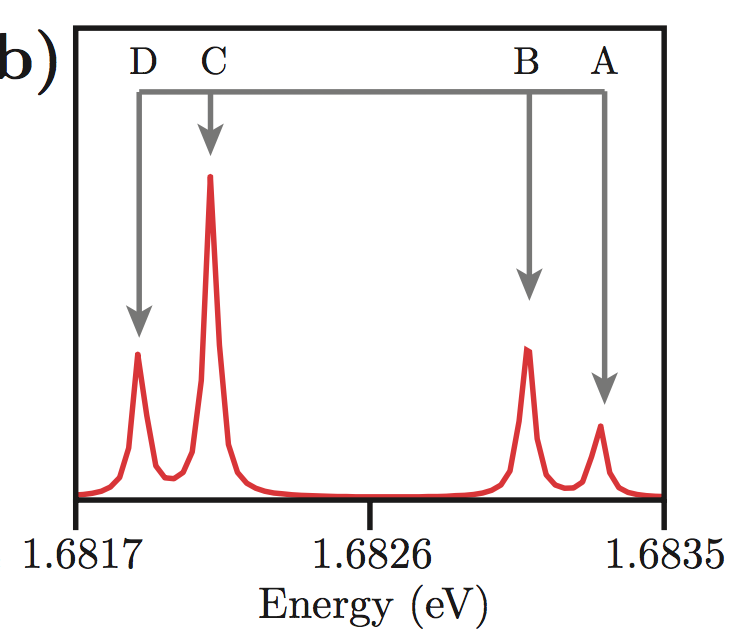
\includegraphics[trim = 0 0 0 0,  clip= true, height = 0.6\textwidth]{./pics/cryogenic_siv.png}}
  			\caption{}
  		\end{subfigure}
  		\caption[Fluorescence spectra of \sivs at low temperature]{(a) Fluorescence spectrum of an ensemble of \sivs at \SI{10}{\kelvin}. $12$ peaks can be seen, $4$ for each stable isotope of silicon \cite{Clark1995}. (b) Fluorescence spectrum of an isolated \siv at \SI{15}{\kelvin}. $4$ peaks can be seen, $2$ for the ground state and $2$ for the excited state. Figure reproduced from \cite{Riedrich-moller2014}.}
  		\label{fig::cryogenic_spectra}
  	\end{figure}
